\documentclass{article}
\usepackage{tikz}
\usepackage{tikz-3dplot}
\usepackage[utf8]{inputenc}
\usepackage[T2A]{fontenc}
\usepackage[russian,english]{babel}
\usepackage{amsmath}
\usepackage{cmap}
\usepackage[a4paper, left=3cm, right=3cm, top=2cm, bottom=2cm]{geometry}
\usepackage{multicol}
\usepackage{caption}
\usepackage[most]{tcolorbox}
\usetikzlibrary{patterns}

\begin{document}
\begin{figure}
\centering
\begin{tikzpicture}
    % Координатная плоскость
    \draw[->] (-6,0) -- (6,0) node[right] {$x$};
    \draw[->] (0,-4) -- (0,4) node[above] {$y$};
    
    % Прямоугольник
    \draw (-4,-3) rectangle (4,3);
    
    % Штриховочные линии
    \begin{scope}
        \clip (0,0) ellipse [x radius=4, y radius=3];
        \draw[dashed] (0,0) -- (-4,-4);
        \draw[dashed] (0,0) -- (4,4);
        \draw[dashed] (2.4,2.4) -- (2.4,-2.4);
        \draw[dashed] (2.4,2.4) -- (-2.4,2.4);
        
    % Овал
    \end{scope}
    
    % Овал
    \draw (0,0) ellipse [x radius=4, y radius=3];
    
    % Подписи точек
    \node at (-2.4,-2.5) [below left] {$(-x,-y)$};
    \node at (2.7,-2.5) [below right] {$(x,-y)$};
    \node at (-2.6,2.5) [above left] {$(-x,y)$};
    \node at (2.9,2.5) [above right] {$(x,y)$};
    \node at (0,0) [above left] {$0$};
    \node at (4,0.4) [below left] {$a$};
    \node at (-4,0.4) [below right] {$-a$};
    \node at (0.6,-3) [above left] {$-b$};
    \node at (0,2.5) [above right] {$b$};
    
    % Подпись рисунка
    \node at (0,-4.5) {\textbf{Рис. 1.} К описанию геометрических свойств эллипса};
\end{tikzpicture}
\end{figure}



\begin{figure}[h]
    \centering
    \begin{tikzpicture}[scale=1.5]
        \fill[pattern=north west lines] (1,1) circle (0.5);
        \draw (1,1) circle (0.5);
        \draw[->] (1,1) -- +(45:0.5) node[midway, above left] {$\delta$};
        \draw[->] (-2,0) -- (2,0) node[right] {$x$};
        \draw[->] (0,-2) -- (0,2) node[above] {$y$};
        \node at (0,0) [below left] {$0$};
        \node at (1,1) [below right] {$z_0$};

        \begin{scope}[shift={(6,0)}]
           
            \draw (0,0) circle (1);
            \fill[pattern=north west lines] (0,0.18) ellipse (1.8 and 1.2);
            \fill[white] (0,0) circle (1);
            \draw[->] (-2,0) -- (2,0) node[right] {$u$};
            \draw[->] (0,-2) -- (0,2) node[above] {$v$};
            \node at (0,0) [below left] {$0$};
            \node at (0,1.3) [below right] {$E$};
            \node at (1,0) [below right] {$E$};
            
        \end{scope}
        
        % Изогнутая стрелка
        \draw[->, bend right=40] (1.3,0.8) to (5,1);
        
        % Подпись фигуры
        \node at (3.5,-2.3) {\textbf{Рис. 4.}  К описанию геометрических свойств (а) и определению параболы (б)};
        
    \end{tikzpicture}
\end{figure}

\begin{figure}[htbp]
    \centering
    \begin{minipage}[b]{0.24\textwidth}
        \centering
        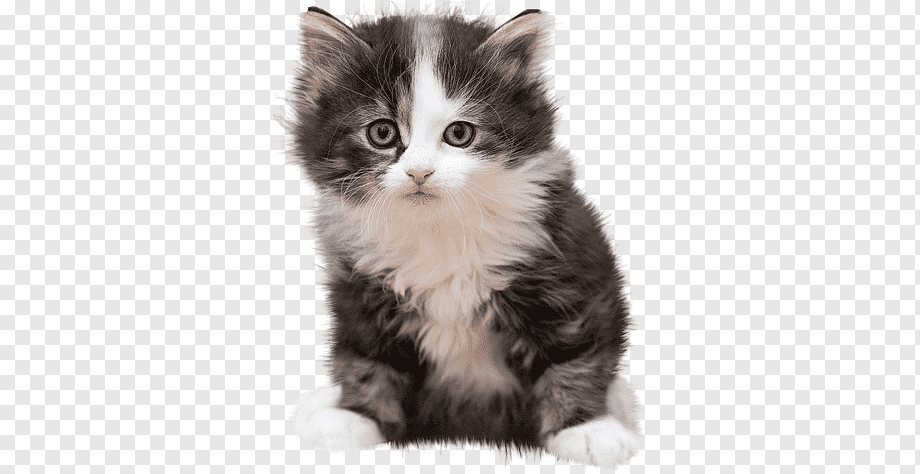
\includegraphics[width=\textwidth]{cat.png}
    \end{minipage}
    \begin{minipage}[b]{0.24\textwidth}
        \centering
        \vspace{0.2cm} 
        \rotatebox{180}{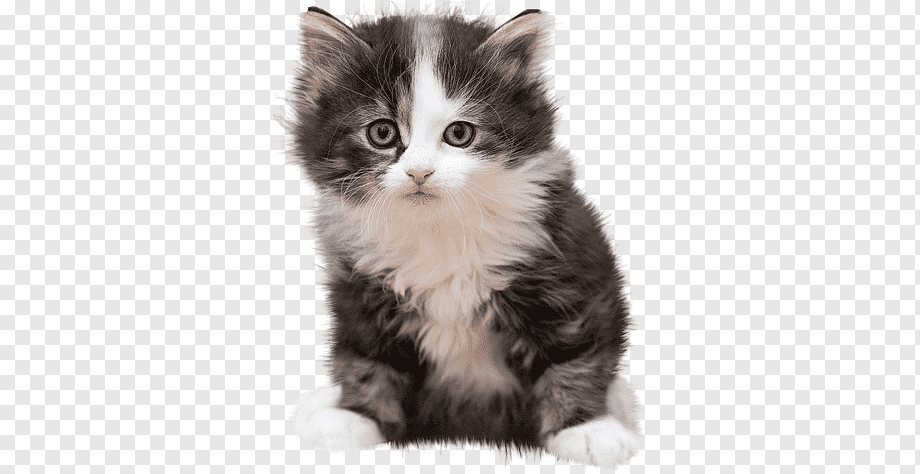
\includegraphics[width=\textwidth]{cat.png}}
    \end{minipage}
    \begin{minipage}[b]{0.1\textwidth} 
        \centering
        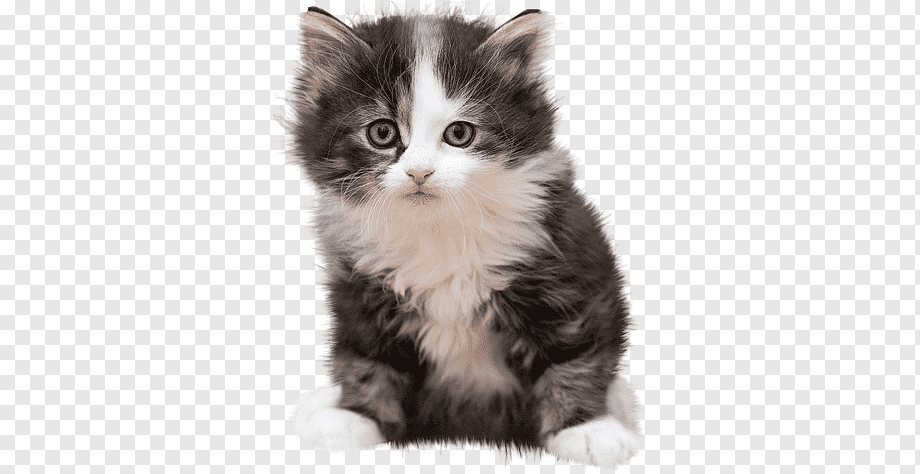
\includegraphics[width=\textwidth]{cat.png} 
    \end{minipage}
    \begin{minipage}[b]{0.1\textwidth} 
        \centering
        \vspace{0.2cm} 
        \rotatebox{180}{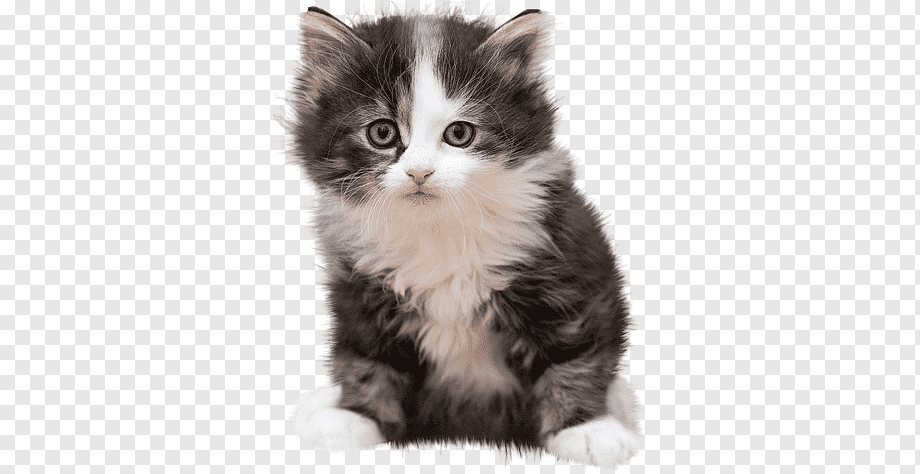
\includegraphics[width=\textwidth]{cat.png}} 
    \end{minipage}
\end{figure}

\begin{figure}
    \noindent
    \begin{minipage}[t]{0.3\textwidth}
        \centering
        \frame{\parbox{\linewidth}{\raggedright \vspace{5pt} bla bla bla bla bla bla bla bla bla bla bla bla bla bla bla bla bla bla bla bla bla bla bla bla bla bla bla bla bla bla bla bla bla bla bla bla bla bla bla bla bla bla  \vspace{5pt}}}
    \end{minipage}%
    \hfill
    \begin{minipage}[t]{0.3\textwidth}
        \centering
        \frame{\parbox{\linewidth}{\centering \vspace{5pt} 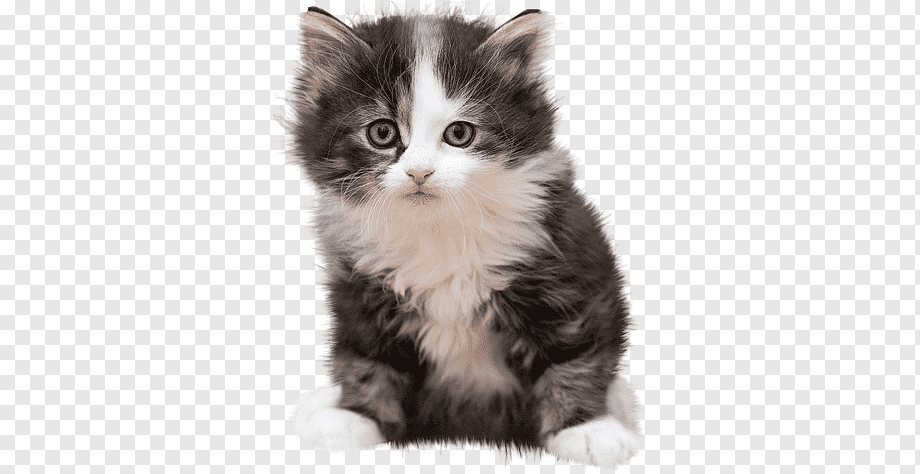
\includegraphics[width=0.8\textwidth]{cat.png}\caption*{Подпись к рисунку} \vspace{5pt}}}
        %\frame - создаёт рамку, \parbox - создаёт саму коробку, \vspace - создаёт пространство между текстом
    \end{minipage}%
    \hfill
    \begin{minipage}[t]{0.3\textwidth}
        \centering
        \frame{\parbox{\linewidth}{\raggedleft \vspace{5pt} bla bla bla bla bla bla bla bla bla bla bla bla bla bla bla bla bla bla bla bla bla bla bla bla bla bla bla bla bla bla bla bla bla bla bla bla bla bla bla bla bla bla  \vspace{5pt}}}
    \end{minipage}
\end{figure}
    
\begin{figure}
    \noindent
    \begin{minipage}[t]{0.45\textwidth}
        \centering
        \frame{\parbox{\linewidth}{\centering \vspace{5pt} 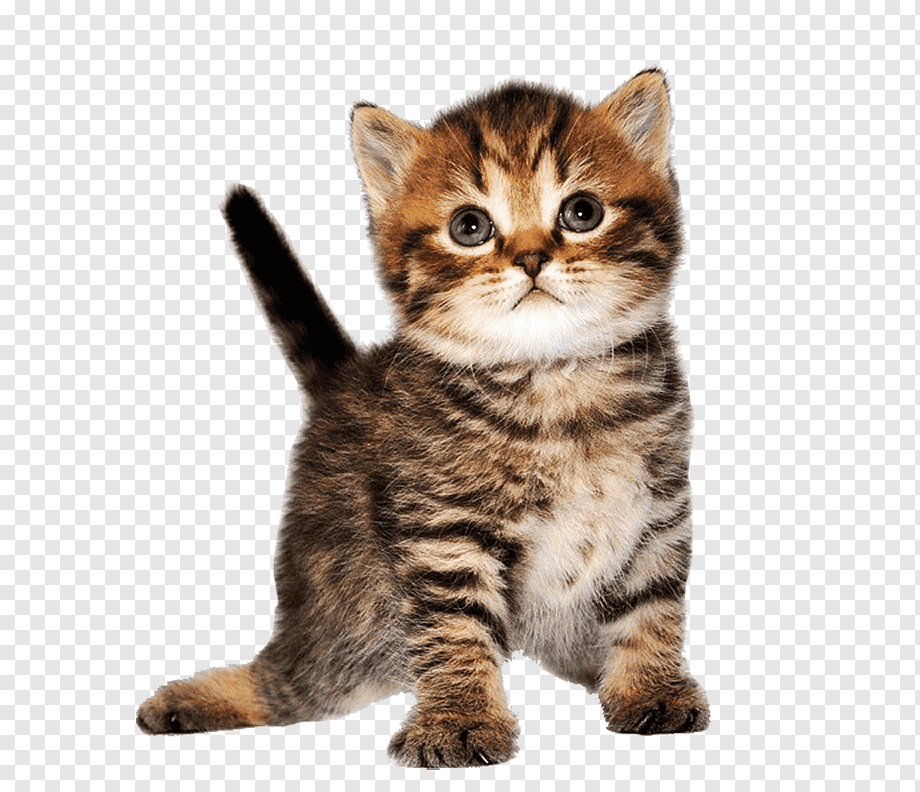
\includegraphics[width=0.8\textwidth]{cat2.png}\vspace{5pt}}}\caption*{котик 1}
        %\frame - создаёт рамку, \parbox - создаёт саму коробку, \vspace - создаёт пространство между текстом
    \end{minipage}%
    \hfill
    \begin{minipage}[t]{0.45\textwidth}
        \centering
        \frame{\parbox{\linewidth}{\centering \vspace{5pt} 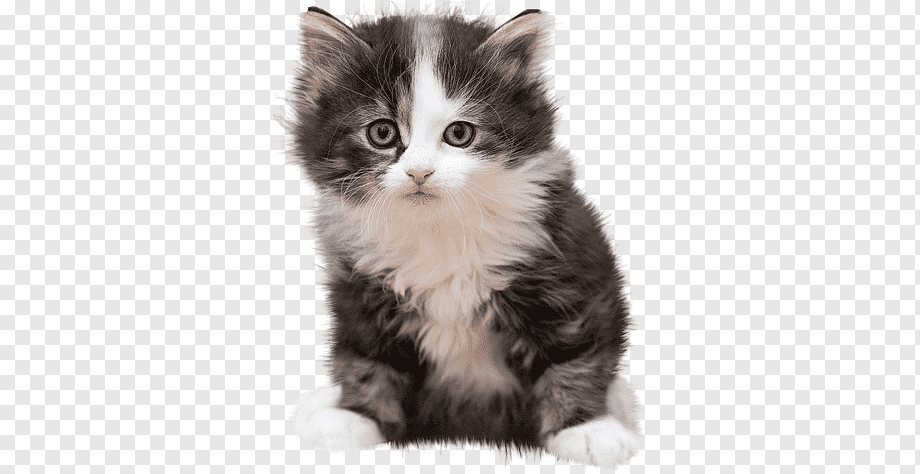
\includegraphics[width=0.8\textwidth]{cat.png}\vspace{5pt}}}\caption*{котик 2}
        %\frame - создаёт рамку, \parbox - создаёт саму коробку, \vspace - создаёт пространство между текстом
    \end{minipage}%
\end{figure}

\end{document}
